Fuzzy sets were introduced by Zadeh in 1965, following the idea of generalizing sets that was presented in section \ref{sec:sorites}:

\say{More often than not, the classes of objects encountered in the real physical world do not have precisely defined criteria of membership. [...]Clearly, the \emph{class of all real numbers which are much greater than 1,} or \emph{the class of beautiful women,} or \emph{the class of tall men,} do not constitute classes or sets in the usual mathematical sense of these terms. [...]Yet, the fact remains that such imprecisely defined \emph{classes} play an important role in human thinking, particularly in the domains of pattern recognition, communication of information, and abstraction.}\cite{Zadeh1965}\\

The idea he proposed for representing those classes is using a continuum of grades of membership. While classical (also called crisp or boolean) sets use a boolean membership function $\chi_A:X\rightarrow\{0,1\}$ that assigns either 0 or 1 to each element, fuzzy sets generalize this by using a membership function $\mu_A:X\rightarrow[0,1]$ that can assign any value between 0 and 1. 

\begin{remark}
    The membership degrees represent how compatible an object is with a set. Since membership degrees are real numbers in $[0,1]$, they are totally ordered. However, this does not imply a total ordering of objects, since two different objects may have the same membership degree. The set of objects can be totally ordered by considering equivalence classes of objects with the same membership degree.
\end{remark}

Let us take a closer look at Zadeh's example of the set of ``tall men" to answer a fundamental question: where do these membership values come from?\\

Most people would agree that a person with a height of 1.50m is not tall, so we can anchor the function with $\mu_{tall}(1.50) = 0$. Conversely, a person 2.00m tall is generally considered tall, so $\mu_{tall}(2.00) = 1$. But how should we define the values in between? The choice is not unique, and this non-uniqueness is not a flaw, but a feature.\\

However, not all choices are valid. For a membership function to be a reasonable model of the ``tall person" concept, it must be consistent with our understanding of it. For example, it would be illogical to define a 1.70m person as taller than a 1.80m person. This means $\mu_{tall}(h)$ must be non-decreasing. Furthermore, a classical boolean definition fails to capture the gradual nature of ``tallness", even if it is not wrong, it lacks the expressive power for more a nuanced definition. Figure \ref{fig:tall_definitions} illustrates these points.

\begin{figure}[!ht]
    \centering
    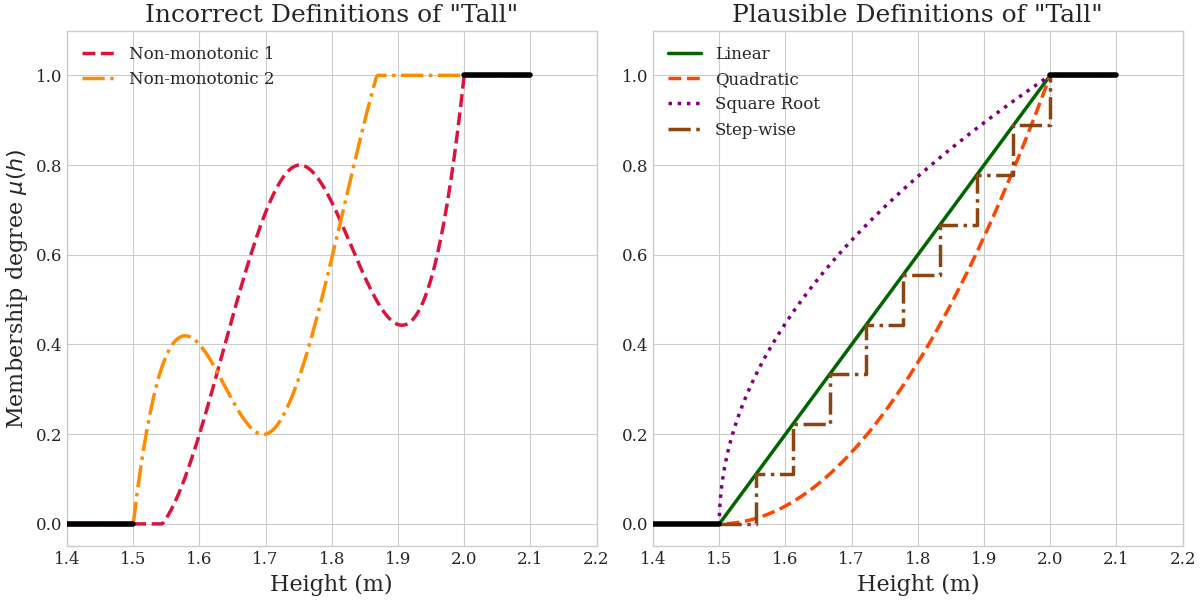
\includegraphics[width=\textwidth]{ch1/figures/Fuzzy_tall.png}
    \caption{Illustrations of different membership functions for the fuzzy set \emph{tall}. The left plot shows incorrect definitions using non-monotonic function which are logically inconsistent since it implies a shorter person could be considered ``more tall" than a taller one. The right plot shows several valid, non-decreasing functions that can represent \emph{tall}. Each reflects a different modeling choice, but all are anchored to the same clear cases: membership is 0 for heights below 1.5m and 1 for heights above 2.0m.}
    \label{fig:tall_definitions}
\end{figure}

As shown in Figure \ref{fig:tall_definitions}, there are (infinitely) many valid ways to define the fuzzy set \emph{tall}. This flexibility might seem like a problem of subjectivity or a lack of rigor, but it is better understood as a matter of definition. In classical set theory, the question is not whether the set of ``natural numbers including zero" is more correct than the set of ``natural numbers starting from one". They are simply different sets defined for different purposes. Similarly, choosing a membership function is the act of defining the fuzzy set. The goal is not to discover a single, universal truth for ``tall people", but to design a fuzzy set that is useful for a specific problem. \\

This allows us to encode context-dependent or domain-specific expert knowledge into a precise mathematical model. The various methods for systematically creating these membership functions, a process known as \textit{fuzzification}, will be discussed in section \ref{sec:fuzzy_aggregation}.\\

For the remainder of this chapter, fuzzy sets will be considered as given, with focus placed on their mathematical properties and operations. Since fuzzy sets extend the concept of crisp sets, every crisp set can be modeled as a fuzzy set while the reverse is not true. The formal definition is presented as follows:

\begin{definition}[Fuzzy Set]
    Let $X\neq\emptyset$ a set. Then we define a \textbf{fuzzy set A in X}, i.e., $A \in \fuzzy{X}$ as:
    \[A=\{(x,\mu_A(x))\mid x\in X\}\]
    Where $\mu_A:X\longrightarrow [0,1]$ is the \textbf{membership function} and $X$ is the \textbf{domain} of the fuzzy set.
\end{definition}

\begin{remark}
     Both the fuzzy set and the membership function uniquely identify each other.
\end{remark}

\begin{notation}{Notation}
    We may use \( A(x) \equiv \mu_A(x) \) interchangeably.

    In general, $\chi$ will denote boolean membership functions and $\mu$, fuzzy membership functions.
\end{notation}



\begin{definition}[Support]
    Let $A \in \fuzzy{X}$. The crisp set of non zero membership value elements is called the support:
    \[\textnormal{Supp}(A)=\{x\in X \mid A(x)>0\}\]
\end{definition}

\begin{definition}[Fuzzy Subset]
    Given the fuzzy sets $A, B \in \fuzzy{X}$ we say $A$ is a fuzzy subset of $B$ (and write $A \subseteq B$) if and only if $A(x)
    \leq B(x) \forall x \in X$.

    Analogously, $A$ and $B$ are equal if and only if $A(x)=B(x) \forall x \in X$, i.e., each of them is a subset of the other.
\end{definition}

\begin{example}
    Here are some examples of common fuzzy sets:
    \begin{itemize}
        \item \textbf{Empty Fuzzy Set in $X$:} such that $\emptyset(x)=0 \forall x \in X$.
        \item \textbf{Universal Fuzzy Set in $X$:} such that $X(x)=1  \forall x \in X$.
        \item \textbf{Fuzzy Point in $X$:} such that $P(x_0)=1 \land A(x)=0 \forall x \in X-\{x_0\}$
        \item \textbf{Fuzzy Number:} Usually defined as a fuzzy set in $\mathbb{R}$ with some desirable properties. Will be covered in section \ref{sec:fuzzy_numbers}.
    \end{itemize}
\end{example}
